\documentclass[a4paper,twocolumn,10pt]{article}
\usepackage[utf8]{inputenc}
\usepackage[english]{babel}
\usepackage{graphicx}
\usepackage{multirow}
\usepackage{tabularx}
\usepackage{array}
\usepackage{geometry}
\usepackage{cuted, ragged2e}
\usepackage{lipsum, array, booktabs, caption}
\usepackage{multirow}
\usepackage{graphicx}

%opening
\title{A Preliminary Analysis of Scratch Projects}

\author{
Ángela Vargas-Alba \\ Universidad Rey Juan Carlos\\
                Madrid, Spain \\ a.vargasa@alumnos.urjc.es
\and
Gregorio Robles \\Universidad Rey Juan Carlos \\
                Fuenlabrada, Madrid, Spain \\grex@gsyc.urjc.es   
}

\date{}


\begin{document}
\maketitle


\small \textbf{\textit{Abstract}—One of the most widely used tools for the initiation in the world of programming is
Scratch, a visual programming language oriented to education. Its use has intensified in the recent years with millions of
projects that can be shared and viewed by other Scratch users. 
In this paper, we analyze a dataset of 250K Scratch projects obtained from the Scratch repository,  with the objective of
extract correlations between different data.}

\begin{center}
\section*\normalsize{I. INTRODUCTION}\\
\end{center}

Presently, increasingly the tendency of introducing the programming in the
classrooms is developing. Nevertheless, there is a lack of formation in this matter and Scratch is a great
usefulness in order to supply this deficiency, due to the fact that, beside helping the educator in the
assessment tasks, it supposes a stimulus to encourage the learners to continue improving their
programming skills. With this tool it is expected to guide the collective in their first steps giving
support, both educators and learners, in the programming sector. \par
In recent years, increasingly the users decide to utilize Scratch as learn programming method. Currently, Scratch
has in its web platform more than 30 millions of shared projects and more than 20 millions of registered users.\par
Thanks to the high activity in the web platform of Scratch, it is possible to inspect different aspects which relate projects
each other. Thus, the motivation of this paper is, on one hand, to analyze which characteristics can relate different projects
and, on the other hand, how metadata of the proyect is related itself, in order to, in a future, this analysis could be
useful for some tools or aplications. \par
In order to accomplish this analysis, we have based on the paper ``A Dataset of Scratch Programs: Scraped, Shaped and
Scored dataset'' [1]. In this work, authors collect data from the web interface of the Scratch project repository, by means 
of a scraping program. It retrieves a JSON file for each of the listed projects and, subsequently, they obtained the JSON files for
250,163 projects. Finally, they parsed this dataset and obtained a   list of Scratch projects with metadata and program data. \par
In this paper, we have utilized this dataset, which contained more than 250K projects from the Scratch repository, with the
main aim of analyze if there is any kind of relationship between them, and extract useful conclusions about it.\par
The structure of the work has been divided according to the following way: In section II. Dataset construction, it will be
developed the process of obtaining the dataset. Section III includes the methodology used to obtain the analyzed correlations.
The results are presented in Section IV and, finally, in the Section V, we present the conclusions reached.

\begin{center}
\section*\normalsize{II. DATASET CONSTRUCTION}
\end{center}

\subsection*\normalsize{\textit{A. Data collection}}\\

To collect the data from the web interface of the Scratch
project repository, we utilized the dataset created by the paper [1].
This dataset was composed as from two files: \textit{metadata.csv} and
\textit{code.csv}. These files were formed by heterogeneous data, that is,
they contained different types of data. For this reason, we initially
did a data filtering. With a script programmed on \textit{python}, we read
both csv files and remove \textit{nul} or ``strange'' values from them.
We understood ``strange'' values as those values that contained some special
characters.\par
Respect to the file \textit{code.csv}, it was a file with large dimensions,
so that we utilized only the 10\% of its content in order to work in a more
comfortable way. This new file, \textit{code\_10\%\_headers.csv},
contained information about only 20,061 of the total projects. For each
project, it contained different data, which will be described in
section B, so that it was formed by 3,988,988 total lines. \par
Based on the filtering process, we removed 3,166 lines, but the number of
different projects was the same, 20,061, so we removed some data related with
projects, but the same number of projects was maintained.\par
On the other hand, we decided to remove the characteristics related to the
parameters of each project. We considered that these data was not relevant
for the analysis, so finally we obtained a file
\textit{code\_10\%\_filt.csv}.\par
Respect to the other file, \textit{metadata.csv}, it was no necessary to carry
out the filtering process. Data of this file was homogeneous, so it was
possible to work directly. However, it contained metadata which we didn't
consider useful in the analysis of this paper. For this reason, we reduce
this file and removed some columns.

\subsection*\normalsize{\textit{B. Data description}}\\

Scratch is a visual programming language whose projects are based on a structure
composed of different blocks. The code of a Scratch program, is formed by scripts,
which is defined as a set of code blocks. Each script belongs to a sprite, an object
with it own associated code. In Figure ~\ref{tab:scratch}, is shown an example
Scratch script witch belongs to a given sprite.

\begin{figure}
\begin{center}
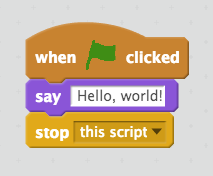
\includegraphics[height=4cm]{images/scratch.png}
\caption{Example of a Scratch program with a script in the same sprite.}
\label{tab:scratch}
\end{center}
\end{figure}

The two files with which we are going to work in this paper are:
\textit{metadata.csv} and \textit{code\_10\%\_filt.csv}. 
The data related with each file is outlined in Table~\ref{tab:schema}.

\begin{table*}
  \centering\renewcommand{\arraystretch}{1.2}
   \begin{tabular}{@{}lccc@{}}
    \toprule
    \multicolumn{1}{c}{\textbf{File}} & \textbf{Key} &\textbf{Attribute(Description)} \\
    \midrule
    \multirow{8}{*}{\textit{code\_10\%\_filt.csv}} & ProjectID & Scratch project Id \\
                & Script-rank & Project-level ranking of script \\
                & Sprite-type & Type of sprite the script is in\\
                & Sprite-name & Name of sprite the script is in\\
                & Coordinates & X-Y location of script in Scratch editor\\
                & Total-blocks & Number of blocks comprising the script \\
                & Line & Script-level ranking of block \\
                & Block-type & Type of block the script is in\\
    \hline
    \multirow{8}{*}{\textit{metadata.csv}} & p\_ID & Scratch project Id \\
                & project-name & Name given to project \\
                & username & Author’s Scratch username\\
                & total-views & Project views number \\
                & total-remixes & Project remixes number \\
                & total-favorites & Total users favoriting \\
                & total-loves & Users ‘loving’ the project \\
                & Mastery & Dr. Scratch total mastery score\\
    \bottomrule
    \end{tabular}
    \caption{Database schema: Data structure and description}
    \label{tab:schema}
\end{table*}

\par In Table~\ref{tab:schema}, the last Key \textit{Mastery}, is the result of Dr. Scratch
score. Dr. Scratch is a web platform of free software or open source that 
allows users to analyze their projects carried out in Scratch, in a simple
way. With Dr. Scratch, both students and educators can analyze if their
projects have been programmed correctly, learn from their mistakes or
receive feedback to improve their code, thus developing their capacity of
Computational Thinking, (CT). \par
In order to assign the punctuation of CT to a certain project, Dr. Scratch
is based on assess the demonstrated level by the programmer in the seven
following aspects: abstraction and decomposition of problems, logical
thinking, synchronization, parallelism, algorithmic notions of flow control, 
interactivity with the user and representation of the information. The 
assessment of each one of these concepts can be 0, 1, 2 or 3 points, being
the projects, therefore, contained in the range from 0 to 21 point. According
to the final punctuation obtained, Dr. Scratch differentiates three levels of
projects: basics, from 0 to 7 points, developing from 7 to 15 points, and
professional, with punctuation between 15 a 21 points.

\begin{center}
\section*\normalsize{III. METHODOLOGY}
\end{center}

One that we had the dataset filtered and ordered, we can analyze them.
The main purpose of the paper is to find correlations among Scratch
projects. In order to reach this objective, we have developed an analysis
process. \par
Initially, we focused on the characteristic "total-blocks". We generated a new
dataset grouped by "projectID", "script-rank" and "total-blocks". In this way,
we obtained the total number of blocks for each Scratch project and its project
Id. The following stage was to analyze among the total blocks of each project, 
which of them were different, that it, we calculated the variety of block types. 
In order to obtain this new characteristic, we grouped the unique block types for
each Scratch project, obtaining a new dataset.\par
We related both dataset and obtained two correlations: the correlation between
"total-blocks" and "variety-blocks", and the correlation between "total-blocks"
and "repeated-blocks", represented in Figure ~\ref{tab:corr_1}. \par


\begin{figure}
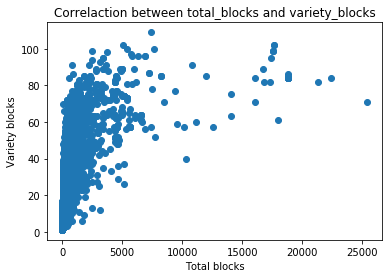
\includegraphics[height=4cm]{images/1.png}
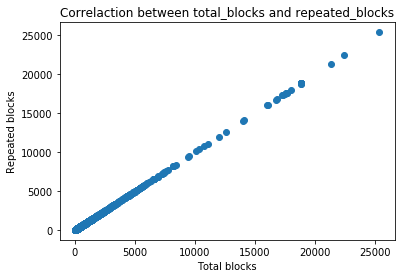
\includegraphics[height=4cm]{images/2.png}
\caption{Correlations between total blocks and blocks type.}
\label{tab:corr_1}
\end{figure}

The following analysis was focused on correlate the total number of blocks per project
and its metadata. For this process, it was necessary relate both CSV files. For this
reason, the first stage was to select from \textit{metadata.csv}, only the id of the
projects contained in file \textit{code\_10\%\_filt.csv}.\par
One that we obtained both files filtered, we analyzed the correlation between 
``total-blocks'' and ``total-views'', ``total-blocks'' and ``total-remixes'', 
``total-blocks'' and ``Mastery'' and ``variety-blocks'' and ``Mastery''. The result
of these correlations is showed in Figure ~\ref{tab:corr_2}.\par

\begin{figure}
\begin{center}
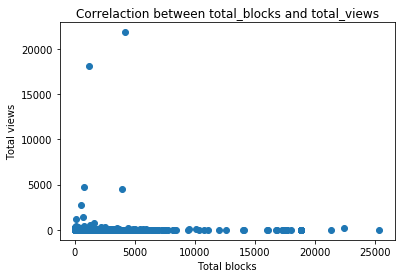
\includegraphics[height=4cm]{images/3.png}
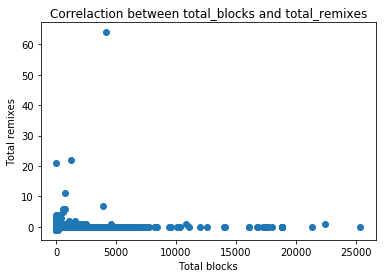
\includegraphics[height=4cm]{images/4.png}
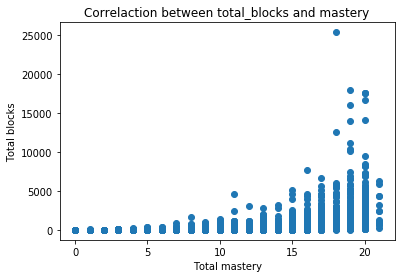
\includegraphics[height=4cm]{images/5.png}
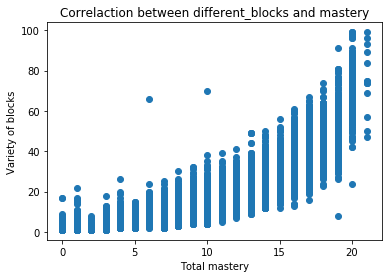
\includegraphics[height=4cm]{images/6.png}
\caption{Correlations between total blocks and metadata.}
\label{tab:corr_2}
\end{center}
\end{figure}

Finally, we considered relevant for the analysis of the paper, to correlate some
characteristics of metadata. In this way, we analyzed the correlation between: 
``Mastery'' and ``total-views'', ``total-remixes'' and ``total-views'',
``total-views'' and ``total-favorites'' and ``total-views'' and ``total-loves''.
The results are represented in Figure ~\ref{tab:corr_3}.

\begin{figure}
\begin{center}
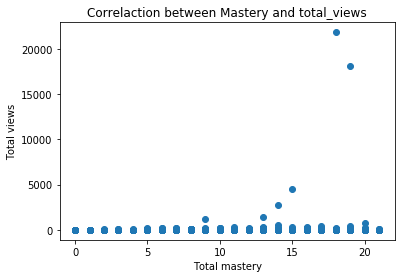
\includegraphics[height=4cm]{images/7.png}
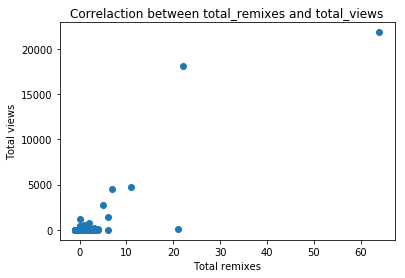
\includegraphics[height=4cm]{images/8.png}
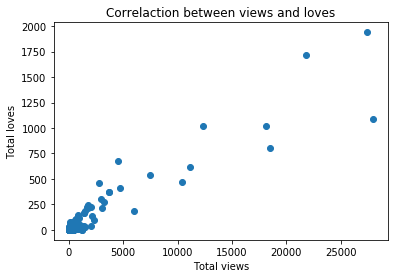
\includegraphics[height=4cm]{images/9.png}
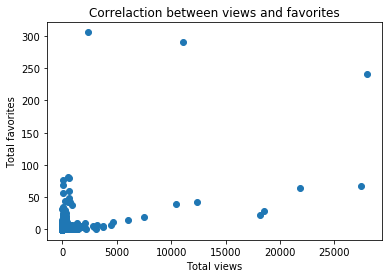
\includegraphics[height=4cm]{images/10.png}
\caption{Correlations between metadata.}
\label{tab:corr_3}
\end{center}
\end{figure}

\begin{center}
\section*\normalsize{IV. RESULTS}
\end{center}

In the first stage of analysis, we obtained interesting results, as is shown in
Figure ~\ref{tab:corr_1}. The value of first correlation is 0.53, which indicates that the 
relation between the number of total blocks in a project is not proportional
to its variety, analyzed as different block types. On the contrary, the
correlation obtained between total blocks in a project and repeated blocks is
0.99. This result indicates that those projects which have a greater number of 
blocks, are formed by more quantity of repeated blocks. \par
In the second analysis, shown in Figure ~\ref{tab:corr_2}, we can observe that it does not exist
a clear correlation between data. These results indicate that projects which have
a greater number of blocks, not necessarily receive a greater number of views and
remixes by other users. On the other hand, projects which have a greater number of
blocks, neither obtain a greater final mastery.\par
Finally, contrary to the previous analysis, Figure ~\ref{tab:corr_3} shows a high correlations 
between metadata of a Scratch project. The correlation obtained between the total
views of a given project and the total number of remixes, is 0.86. This result 
indicates that those projects that have realized a greater quantity of remixes,
are more socials and receive a greater quantity of views. If we analyze the 
correlation between total views of a project and its total number of loves and
favorites, the correlation is even greater. The results obtained, correspondingly
are 0.94 and 0.95. That is, whose projects that have received a greater number
of views, will receive more favorites and loves of other users. However, the
correlation between total views and the final mastery of a project, is almost
null. Projects with more views, not necessarily will have a greater mastery.\par
In Table ~\ref{tab:values}, is shown a summary of the obtained results.

\begin{table}
   \begin{tabular}{@{}lccc@{}}
    \toprule
    \multicolumn{1}{c}{\textbf{Attributes}} &\textbf{Correlation} \\
    \midrule
	Total-blocks, Variety-blocks & 0,53\\
        Total-blocks, Repeated-blocks & 0,99\\
        Total-blocks, Total-views & -0,01\\
        Total-blocks, Total-remixes & -0,01\\
        Total-blocks, Mastery & -0,01\\
        Variety-blocks, Mastery & -0,02 \\
        Mastery, Total-views & 0,03\\
        Total-remxies, Total-views & 0,86\\
        Total-views, Total-loves & 0,94\\
        Total-views, Total-favorites & 0,95\\
    \bottomrule
    \end{tabular}
    \caption{Summary of obtained correlations}
    \label{tab:values}
\end{table}

\begin{center}
\section*\normalsize{V. CONCLUSIONS}
\end{center}

We presented an analysis of data obtained from Scratch projects repository, thanks
to the previous work of the paper [1], which includes the source code of the Scratch
projects, their metadata, and their programming mastery scoring results.
After a filtering process, we obtained the dataset analyzed in this paper. We
searched different correlations between code source of a Scratch project and metadata.
The analysis performed can facilitate the development of some applications or tools
in education area and computing assessment.

\begin{center}
\section*\normalsize{REFERENCES}
\end{center}

\small{[1]	E.Aivaloglou, F.Hermans, j.Moreno-León and G.Robles, ``A Dataset of Scratch Programs:
Scraped, Shaped and Scored'', Report TUD-SERG-2017-007.}
\end{document}
